\chapter{Theoretical Aspects}
\label{cha:theorethicalAspects}

In this chapter, I would like to describe a theory standing behind my work and its use nowadays.

\section{State of the Art}
\label{sec:stateOfTheArt}

Nowadays, broadly understood data becomes one of the most desired resources; everyone wants to research everything. For example, many mobile applications want their user to access localization or send some information to servers. However, the more data we have, the more time it requires from human to process it and extract only things we need. Top it all off it needs to be interpreted afterwards to make some sense of it. That is why Data Science \cite{dataScience} becomes so popular these days. It tries to solve the problem of growing time taken to process bigger and bigger sets of data. The solution turned out to be simple --- "let the machines do the work". That is how Machine Learning (ML) was born. Computer Vision \cite{cv} (CV) in the other hand is an Artificial Intelligence (AI) branch specified for working with image/video, and it uses ML algorithms as a step to achieve its goals of extracting needed data from images/videos with as little human work as possible. It uses Evolutionary Computing \cite{cv} to \textit{"obtain visual functions from video"} \cite{cv} and more specifically, it bases its Pattern Recognition \cite{cv} on this Computing. As of today, CV finds more and more application in various science branches. The most known use of CV is the development of Autonomous Driving. There is also technology for monitoring and prevention of pests and grass diseases \cite{appResearch}, based on CV. Also as an example, China's government works on the spread of street cameras with face recognition software, but that is less of a positive example as some would say, used for human behaviour control. However, in my knowledge, there is no Visual Bicycle Counter in a commercial application.

\section{What a Bicycle Counter Is and Why Make It "Visual"}
\label{sec:why}

As the name suggests, Bicycle Counter is a device for counting cyclists driving by a specific street or bike path. Usually, it is a convection loop embedded in the asphalt of a road, but photocells installed by the roadside are becoming more popular. Both devices count cyclists passing by and save the number on some server, to make it accessible to obtain for authorized people. That information can later serve as a good indicator of bicycle traffic in the city. In Figure \ref{fig:countersKrakow} we can see that there are 17 of those devices installed across the city and numbers from them are publicly available in Krakow.
\begin{figure}[H]
    \centering
    \resizebox{\textwidth}{!}{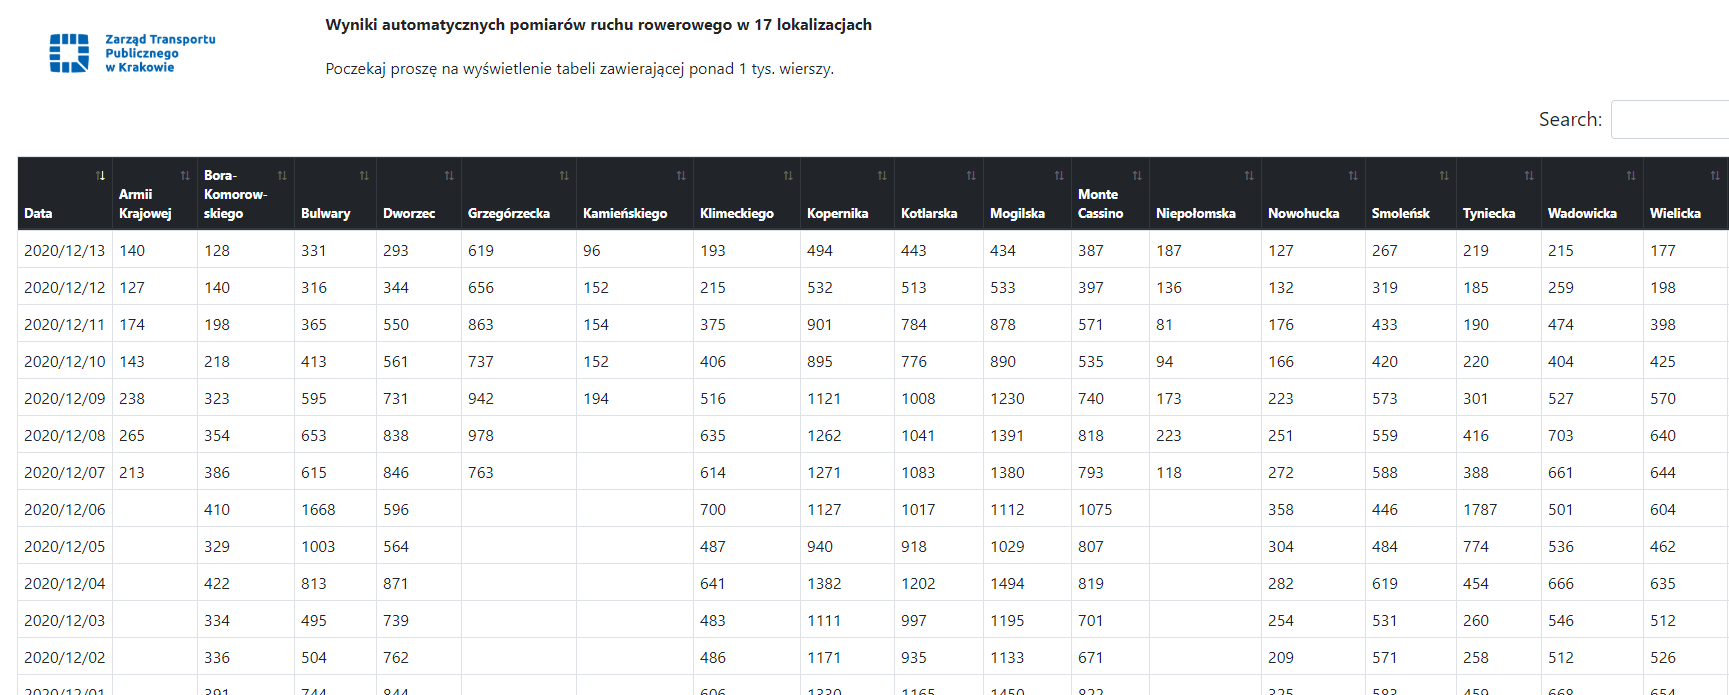
\includegraphics{images/countersKrakow}}
    \caption{First rows of data from bicycle counters installed in Krakow \cite{liczniki}}
    \label{fig:countersKrakow}
\end{figure}
Devices like this will be more and more needed as more and more bicycles appear on streets. Using data from the oldest Bicycle Counter installed in Krakow  \cite{liczniki} we can see that number of cyclists grows slowly but surely in recent years (Figure \ref{fig:graph3}) what can alarm local government to make additional investments like new bike roads.
\begin{figure}[H]
    \centering
    \resizebox{\textwidth}{!}{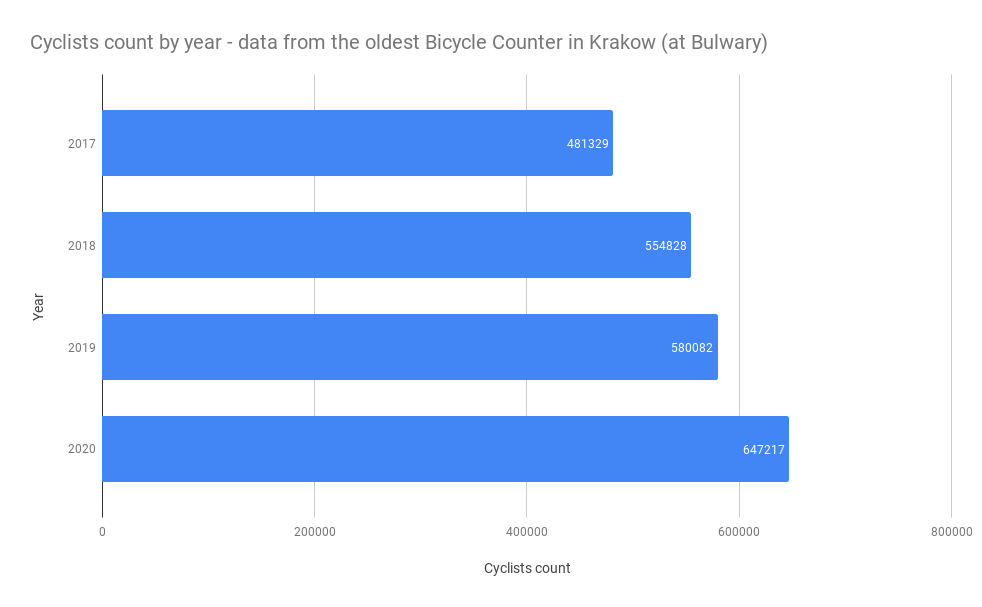
\includegraphics{images/graph3}}
    \caption{Cyclists count at Bulwary, Krakow}
    \label{fig:graph3}
\end{figure}
But why even bother about making Visual Bicycle Counter? First of all, devices I mentioned above are all other equipment used with only one purpose --- counting cyclists, so their reusability leaves a lot to be desired. Secondly, installing such a device requires to put more work into it, because you need to, for example, make a hole in the road, put a convection loop in and patch the hole up. Same as maintenance can be problematic too. Visual Bicycle Counter could solve those issues. It uses a trained ML model to perform inference on video files from street cameras downloaded on a computer or straight on video streams from websites that publicly share it. That would not add the next device but would use street cameras' existing infrastructure, widely developed in many cities.

\section{Short Theory Behind Visual Bicycle Counter}
\label{sec:theory}

Visual Bicycle Counter bases on deep learning model \cite{deepLearning}, what has an advantage over traditional target detection. "The traditional method is to manually extract features and require experts in related fields to manually design and process them through years of accumulation and experience. The method of deep learning can learn the features of difference in response data through a large amount of data and is more representative. The deep learning model simulates the human brain's visual perception system. It extracts features directly from the original image, and the features are passed through the layer by layer to obtain the high-dimensional information of the image, making it a great success in the field of computer vision." \cite{deepLearning}, But first I had to train my model after collecting data to create a dataset for training (in my case: label video frames --- show precisely where the cyclist is, divide labelled frames to train and test). Training the model is "showing" computer training data, it learns those and based on what is learns it tries to predict desired information on test data and then the process is repeated many, many times until reaching satisfactory parameters. For me, the primary metrics were: Loss, Recall, Precision. Loss is a target function minimized in the optimization process (the lower, the better, and it gets lower when the model predicts more accurately). Recall means how many of the relevant items was selected, and Precision means how many selected items are our desired items. Visualization of Recall and Precision is shown in Figure \ref{fig:RPL}.

\begin{figure}[H]
    \centering
    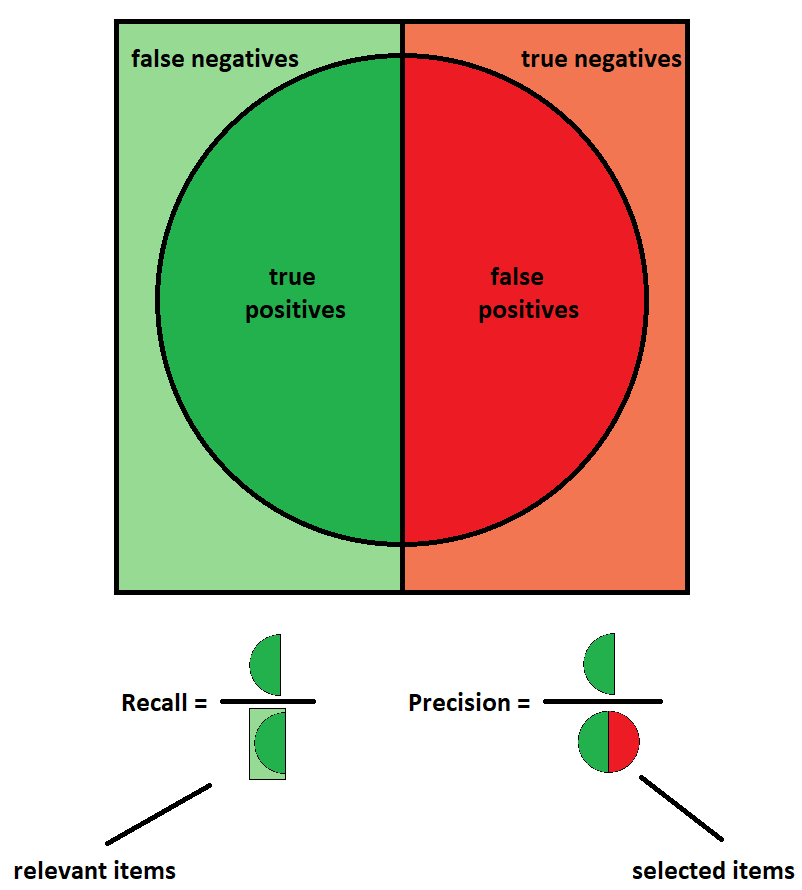
\includegraphics[scale=0.5]{images/rpl}
    \caption{Recall and Precision}
    \label{fig:RPL}
\end{figure}

\section{Tools Selection}
\label{sec:tools}

Tools I have used to create my Visual Bicycle Counter were as follow:
\begin{itemize}
    \item youtube-dl software for downloading video streams from street cameras as mp4 files
    \item LabelImg program for manual image labelling 
    \item Virtual Machine with Ubuntu 18.04.5 LTS for download scheduling 
    \item Google Colaboratory as working environment,
    \item Python programming language,
    \item OpenCV libraries for object detection (used by YOLOv5 API),
    \item YOLOv5 API for training YOLO \cite{Redmon_2016_CVPR} models and performing inference,
    \item Wandb for training evaluation.
\end{itemize}
Most of the choices were pretty obvious. I was looking for widely used solutions that provide good documentation and a big user base. Youtube-dl was the easiest tool to install and use. Using Google Colaboratory (GC) machine was not only my choice but at a certain stage of work, I needed a more powerful GPU and CPU. GC provided all that as well as Python programming language support. The biggest challenge appeared when I was looking for Object Detection tools. I had to test different solutions, such as Tensorflow with Keras, but I found it not suitable for my use case, so I decided to use OpenCV libraries, YOLOv5 API and Wandb that appeared much more user friendly and provided all features I needed.
